\documentclass{beamer}
\usepackage{fprog}

\title{Основни понятия в Haskell}

\date{16 декември 2015 г.}

\begin{document}

\begin{frame}
  \titlepage
\end{frame}

%\includeonlyframes{current}

\section{Въведение в Haskell}

\begin{frame}
  \frametitle{Какво е Haskell?}
  \pause
  \begin{center}
    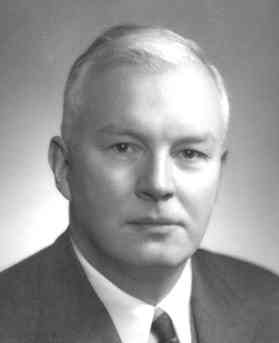
\includegraphics[height=4cm]{images/HaskellBCurry.jpg}\\
    Haskell Brooks Curry\\
    (1900--1982)
  \end{center}
\end{frame}

\begin{frame}[fragile]
  \frametitle{Какво е Haskell?}
  \pause
\begin{verbatim}
fact 0 = 1
fact n = n * fact (n-1)
\end{verbatim}
  \pause
\begin{verbatim}
quickSort []     = []
quickSort (x:xs) = filter (<=x) xs ++ [x] ++ filter (>x) xs
\end{verbatim}
  \pause
\begin{verbatim}
студенти = [("Иван", 40000, 3.5), ("Мария", 60001, 5.5),
            ("Петър", 40002, 5.0), ("Галя", 40003, 4.75)]
избрани = tail (foldr (++) [ ' ':име | (име, фн, оценка) <- оценка,
                                       оценка > 4.5, фн >= 40000 ])
\end{verbatim}
\end{frame}

\begin{frame}
  \frametitle{Какво е Haskell?}
  \pause
  \begin{itemize}
  \item Чист функционален език (без странични ефекти)
  \item Статично типизиран с автоматичен извод на типовете
  \item Използва нестриктно (лениво) оценяване
  \item Стандартизиран (Haskell 2010 Language Report)
  \end{itemize}
\end{frame}

\begin{frame}
  \frametitle{Помощни материали}
  \begin{enumerate}
  \item S. Thompson. Haskell: The Craft of Functional Programming (2nd ed.). Addison-Wesley, 1999.
  \item P. Hudak, Peterson J., Fasel J. A Gentle Introduction to Haskell 98, 1999 (Internet, 2008).
  \item Haskell Wiki: \url{https://wiki.haskell.org/Haskell}
  \item Haskell Platform: \url{https://www.haskell.org/platform/}
  \end{enumerate}
\end{frame}

\section{Дефиниции}

\begin{frame}
  \frametitle{Синтактични елементи}
  \begin{itemize}
  \item Идентификатори: \tt{fact}, \tt{\_myvar}, \tt{студенти}
    \begin{itemize}
    \item имена на обекти, започват с малка буква или \tt\_
    \end{itemize}
  \item Запазени идентификатори: \tt{case}, \tt{if}, \tt{let}, \tt{where}, \ldots
  \item Конструктори: \tt{Integer}, \tt{Maybe}, \tt{Just}, \ldots
    \begin{itemize}
    \item имена на конструкции, започват с главна буква
    \end{itemize}
  \item Числа: \tt{10}, \tt{-5.12}, \tt{3.2e+2}, \tt{1.2E-2}, \tt{0x2f}, \tt{0o35} 
  \item Операции: \tt+, \tt*, \tt{\&\%}, \tt{<==>}, \tt{$\spadesuit$}
    \begin{itemize}
    \item поредица от символи (без букви и цифри)
    \item всички операции с изключение на унарния \tt- са инфиксни
    \end{itemize}
  \item Запазени операции: \tt{..} \tt: \tt{::} \tt= \tt\textbackslash \tt| \tt{<-} \tt{->} \tt@ \tt\~ \tt{=>}
  \item Специални символи: \tt( \tt) \tt, \tt; \tt[ \tt] \tt` \tt\{ \tt\}
  \item Знаци: \tt{'a'}, \tt{'\textbackslash n'}, \tt{'+'}
  \item Низове: \tt{"Hello, world!"}, \tt{"произволен низ"}
  \end{itemize}
\end{frame}

\begin{frame}
  \frametitle{Декларации}
  
\end{frame}

\begin{frame}
  \frametitle{Типове}
  
\end{frame}

\end{document}